\chapter{Mixed Precision Jacobi Algorithm}\label{chap:mixed-precision}

In this chapter, a mixed precision algorithm will be presented with intensive testings on its convergence, speed and accuracy. As mentioned in the Section~\ref{sec:test-matrices}, we will perform the testings for both mode \inline{'geo'} and mode \inline{'ari'}. 

\section{Algorithm}\label{sec:precondition-algorithm}

As discussed from~\ycite[2000]{DRMAC2000-preconditioner}, we can improve the Jacobi algorithm by using a preconditioner. From the discussions in Chapter~\ref{chap:jacobi_algorithm} and~\ref{chap:orthogonalisation}, we assemble them all and collapse into the following algorithm,
\begin{algorithm}[ht]
  \caption{(\textit{Mixed precision Jacobi algorithm}) Given a symmetric matrix $A\in\R\nn$ and a positive tolerance $tol$, this algorithm computes the eigendecomposition of $A$ using the cyclic-by-row Jacobi algorithm with preconditioning.}
  \label{alg:jacobi-preconditioned}
  \begin{algorithmic}[1]
    \State{Compute the eigendecomposition in single precision, $A = Q_\ell D_\ell Q_\ell\tp$.}
    \State{Orthogonalize $Q_\ell$ by using the Newton--Schulz iteration as shown in the Algorithm~\ref{alg:NSiter2}, and we have the output $Q_d$.}
    \State{Precondition $A$ via $A_{\text{cond}} = Q_d\tp A Q_d$ and apply the cyclic-by-row Jacobi algorithm on $A_{\text{cond}}$ to get the orthogonal matrix $V$ and the diagonal matrix $\varLambda$ such that $V\varLambda V\tp = A_{\text{cond}}$.}
    \State{Output the diagonal matrix $\varLambda$ and the orthogonal matrix $Q = Q_d V$ such that $A = Q\varLambda Q\tp$.}
  \end{algorithmic}
\end{algorithm}

\subsection{Implementation and Testing}\label{sec:ref111}

It is straightforward to implement Algorithm~\ref{alg:jacobi-preconditioned} by utilizing the existing codes. MATLAB code can be found in Appendix~\ref{app:mixed-precision-jacobi}. 

We would like to first access its accuracy concerning both the dimension and the condition number. Using code in Appendix~\ref{app:precondition-accuracy} we can produce Figure~\ref{fig:precondition-accuracy}. 


\begin{figure}[ht]
  \centering
  \includegraphics[width=0.85\textwidth]{figs/accuracy_precondition.pdf}
  \caption[Behavior of the relative error $\norm{AQ-Q\varLambda}/\norm{A}$ where $A\in\R\nn$ is symmetric and $Q$ and $\varLambda$ are the results computed using Algorithm~\ref{alg:jacobi-preconditioned}.]{Behavior of the relative error $\norm{AQ-Q\varLambda}/\norm{A}$ with the dimension $n$ and the condition number $\kappa(A)$ increases. The matrices for the testings on the blue line have geometrically distributed singular values and those on the red line have arithmetically distributed singular values. The black line is the reference tolerance $nu_d$.}
  \label{fig:precondition-accuracy}
  \end{figure}
  

As shown from the figure, the Algorithm~\ref{alg:jacobi-preconditioned} gives more accurate results for the matrices with geometrically distributed singular values. But regardless of the distributions, the computed $Q$ and $\varLambda$ satisfies the condition 
\begin{equation}\notag
  \norm{AQ - Q\varLambda} \lesssim nu_d\norm{A},
\end{equation}
and therefore this algorithm can be used to find the eigendecomposition of a real symmetric matrix in practice. The remaining of this chapter is to find out two things
\begin{enumerate}
  \item How many sweeps of Jacobi will be necessary for convergence for a preconditioned real symmetric matrix $A_\text{cond}$ as described in Algorithm~\ref{alg:jacobi-preconditioned}?
  \item How much time can be saved by using preconditioning?
\end{enumerate}

\section{Convergence and Speed}

In this section, we will analyze how many sweeps will be sufficient for the cyclic-by-row Jacobi algorithm converges for a preconditioned symmetric matrix $A_{\text{cond}}$.

\subsection{Preconditioning}\label{p3:sec:precondition}

Using the notations from Algorithm~\ref{alg:jacobi-preconditioned}, $Q_d$ is the nearest orthogonal matrix compare to the approximate eigenvector matrix $Q_\ell$, hence $A_{\text{cond}}$ is expected to be almost diagonal. Consequently, we expect this eigenvalue problem should be able to be solved more quickly by the Jacobi algorithm \ycite[2000, Sec.~1, Corollary~3.2]{DRMAC2000-preconditioner}. Quantitatively, after preconditioning, the magnitude of the off-diagonal entries of $A_\text{cond}$ should be no more than $nu_\ell \norm{A}$, which is equivalently saying $\off(A_\text{cond}) \lesssim n^2(n-1)u_\ell \norm{A}$. In practice, this bound is sharper than the theoretical bound and we can have 
\begin{equation}\label{p3:eq:offAbound}
  \off(A_\text{cond}) \lesssim nu_\ell \norm{A}.
\end{equation}

This upper bound can be numerically tested by the following procedure: First, generate a symmetric matrix $A\in\R\nn$ with controlled dimension and condition number, then we perform steps 1,2 and 3 in the Algorithm~\ref{alg:jacobi-preconditioned} to see how much $\off(A)$ is reduced based on this precondition technique. Using the code in Appendix~\ref{p3:sec:figure1}, we generate Figure~\ref{p3:fig:approx-eig-test}.

\begin{figure}[ht]
\centering
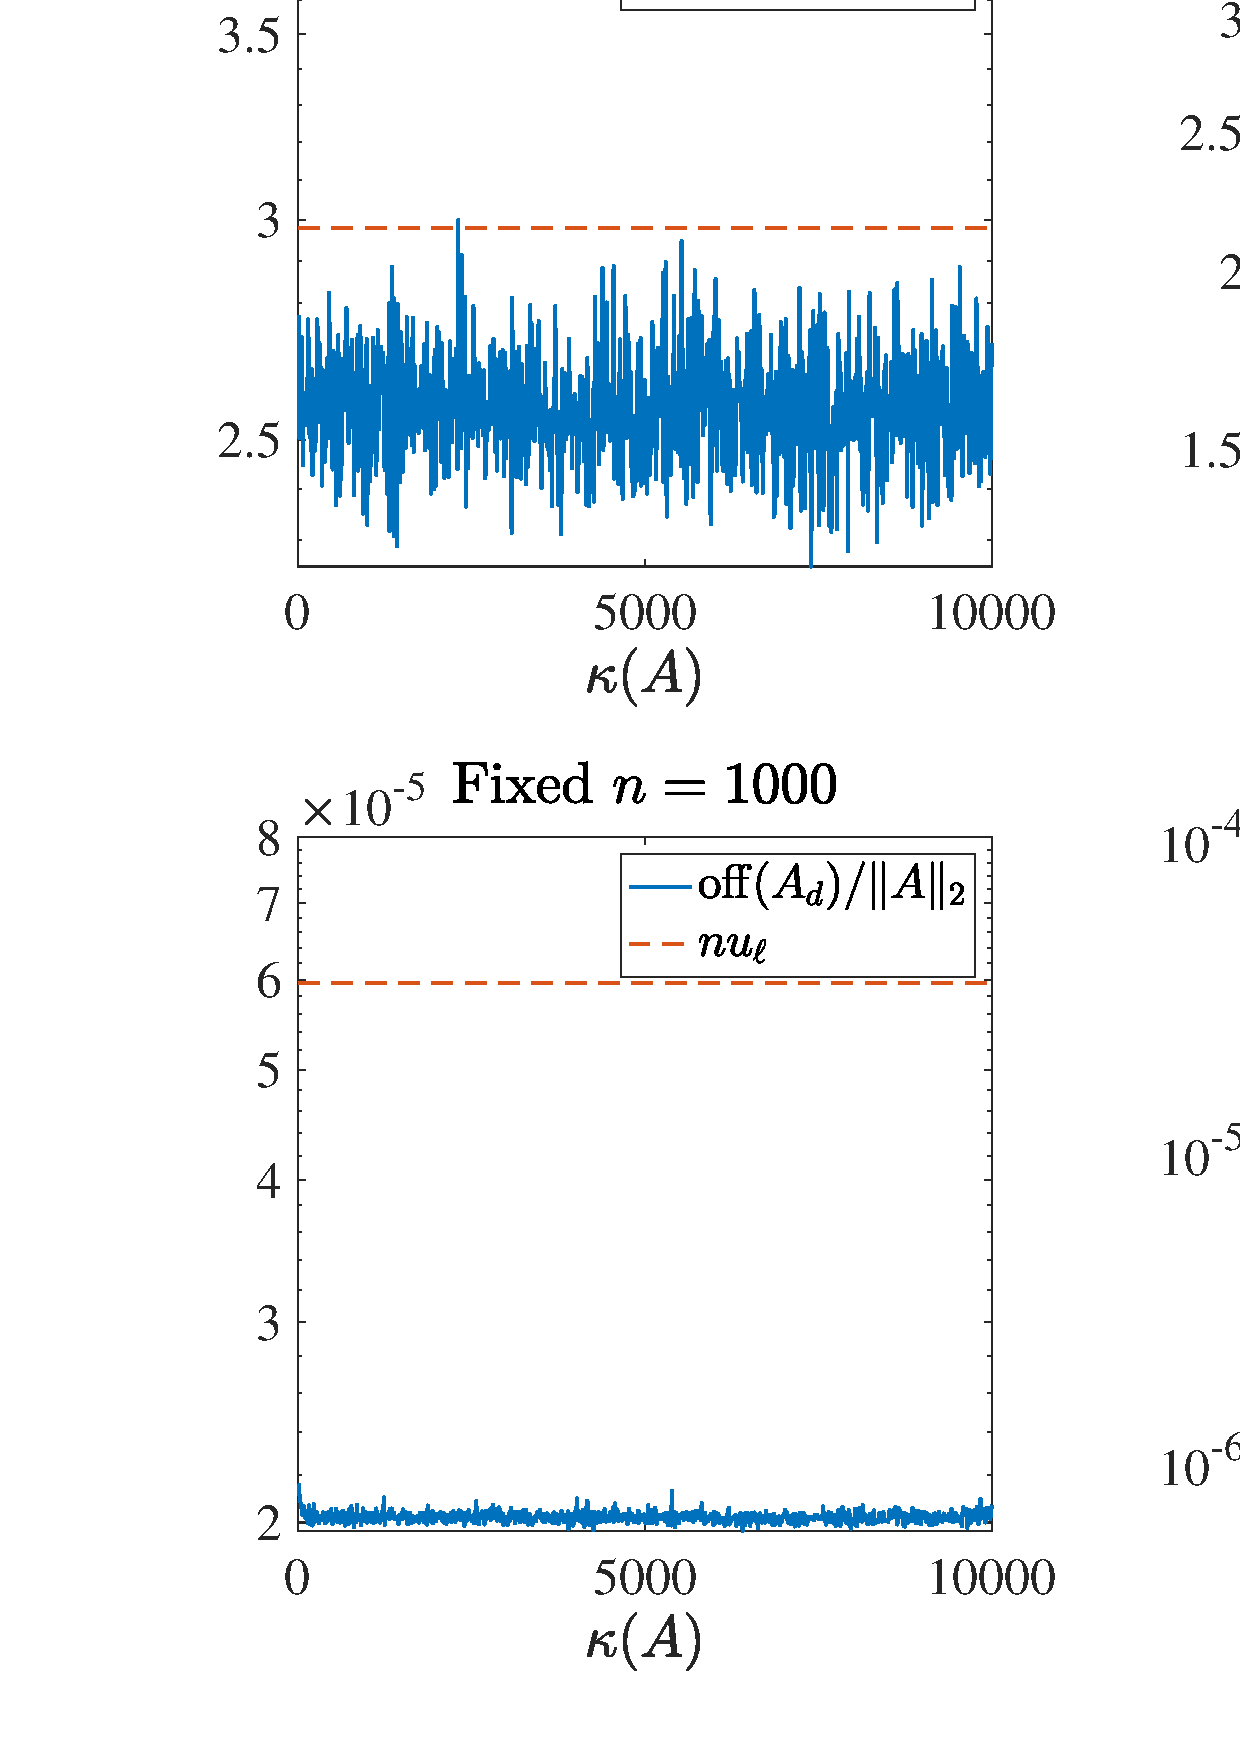
\includegraphics[width=0.8\textwidth]{figs/approx-eig.pdf}
\caption[Four comparisons of $\off(A_\text{cond})/\norm{A}$ with the reference line $nu_\ell$ where $A_\text{cond}$ is the preconditioned matrix described in the Algorithm~\ref{alg:jacobi-preconditioned}.]{Top-left, Top-right, Bottom-left: These figures show the $\off(A_\textup{cond})/\norm{A}$ for $A\in\R\nn$ with different condition number while fixing $n = 50, 250$ and $500$ respectively and varying $\kappa(A)$ from $10$ to $10^3$. Bottom-right: This figure shows the $\off(A_\textup{cond})/\norm{A}$ for $A\in\R\nn$ with different $n$ while fixing $\kappa(A) = 100$ and varying $n$ from $10$ to $1000$. The blue and red line represent the testings on the real symmetric matrices with geometrically and arithmetically distributed singular values respectively.}
\label{p3:fig:approx-eig-test}
\end{figure}

From the top-left, top-right and bottom-left parts of the Figure~\ref{p3:fig:approx-eig-test}, we see that for $n=50,250$ and $500$, the quantity $\off(A_\text{cond})/\norm{A}$ is always smaller or similar to $nu_\ell$ regardless of its singular values distribution. Notice that, as $n$ changes from $50$ to $500$, the perturbation of the quantity $\off(A_\text{cond})/\norm{A}$ becomes more and more negligible compare to $nu_\ell$. Together with the bottom-right figure, as the size of $A$ passes $100$, the quantity $\off(A_\text{cond})/\norm{A}$ is always well bounded by $nu_\ell$. Based on these observations, we verify the idea of preconditioning and prove numerically that after preconditioning $A$ by $Q_d\tp A Q_d$, the off-diagonal entries are reduced significantly and this property can be captured by the Jacobi algorithm.



\subsection{Quadratic Convergence}\label{sec:quadratic-conv}

Based on the preconditioning process, in this section, we will discuss the convergence of the cyclic Jacobi algorithm applied to a preconditioned real symmetric matrix. Then we will deliver some numerical testings concerning different dimensions and condition numbers. Finally, we will test the improvements in speed by using the preconditioners.

Recall that the number of iterations in one sweep is equal to half of the number of off-diagonal entries,
\begin{equation}\notag
  \text{one sweep of $A$} = \frac{n(n-1)}{2},\quad A \in\R\nn.
\end{equation}

From the previous derivation, the Jacobi algorithm is proved to converge linearly. However, an improvement by Sch{\"o}nhage in 1961~\ycite[1961]{1961-first-quadratic-convergence-Schu} stated that the Jacobi algorithm for symmetric matrices with distinct eigenvalues is converging quadratically. Let us denote $A\iter{k}\in\R\nn$ be the matrix produced by the $k$th iteration of the Jacobi algorithm and therefore $A\iter{0}\in\R\nn$ is the original input matrix. Denote $\lambda_1,\dots,\lambda_n$ be the eigenvalues of $A\iter{0}$ and suppose we have 
\begin{equation}
  \label{p3:eq:eig-distance}
  \abs{\lambda_i - \lambda_j} < 2\delta,\quad i\neq j.
\end{equation}

Suppose we reach the stage that the $\off(A\iter{k}) < {\delta}/{8}$ and the angles of rotation generate by each iteration are smaller than $\pi/4$, as controlled in Section~\ref{sec:2.3}, Sch{\"o}nhage's result said 
\begin{equation}\notag
  \off(A\iter{N+k}) \leq \frac{n\sqrt{(n-2)/2}}{\delta}\off(A\iter{k})^2,\quad N = \frac{n(n-1)}{2},
\end{equation}
which implies quadratic convergence. Later in 1962, Wilkinson provided a sharper bound~\ycite[1962, Section~3]{1962-quadratic-convergence-Jame_Wilkinson}. Under the same condition as described by Sch{\"o}nhage, Wilkinson proposed
\begin{equation}\notag
  \off(A\iter{N+k}) \leq \off(A\iter{k})^2 /\delta.
\end{equation}

In 1966, van Kempen proved the quadratic convergence without the assumption of distinct eigenvalues. In his paper~\ycite[1966, Section~2]{1966-quadratic-convergence-vanKempen}, instead of define $\delta$ as in \eqref{p3:eq:eig-distance}, he denoted $\delta$ as 
\begin{equation}
  \label{p3:eq:eig-value-dist-legit}
  \min_{\l_i \neq \l_j} \abs{\l_i - \l_j} \geq 2\delta.
\end{equation}
Suppose after $k$ iterations, $\off(A\iter{k}) < \delta/8$, then 
\begin{equation}\notag
  \off(A\iter{k+N}) \leq \frac{\sqrt{\frac{17}{9}}\off(A\iter{k})^2}{\delta}
\end{equation}
Note that although the above bound is correct, the proof in~\ycite[1966]{1966-quadratic-convergence-vanKempen} is not correct. This mistake was unveiled by Hari who proposed a sharper bound~\ycite[1991, Section~2]{hari_sharp_1991}.

Back to our situation, as described in Section~\ref{p3:sec:precondition}, after preconditioning, $\off(A) \lesssim nu_\ell \norm{A}$. Assuming our eigenproblem is well conditioned and the minimum distance between the distinct eigenvalues is large enough such that 
$$\off(A) \lesssim 0.1 < \delta / 8$$
where $\delta$ is defined by~\eqref{p3:eq:eig-value-dist-legit}. Then we can expect quadratic convergence and the number of iterations should not exceed five since it will only take $4$ sweeps for the quantity $\off(A)$ reduces from $0.1$ to $10^{-16}$ ($0.1^4 = 10^{-16}$).

\subsection{Numerical Testing}
By referring to the function \inline{jacobi_precondi} in Appendix~\ref{app:mixed-precision-jacobi}, we can output the number of iterations required. Therefore, we can investigate the number of sweeps required using the routine from Appendix~\ref{app:typical-sweep}. The procedure is exactly the same as the testing in Section~\ref{sec:ref111} and we can produce Figure~\ref{fig:typical-sweep}.

\begin{figure}[ht]
\centering
\includegraphics[width=0.8\textwidth]{figs/typical-sweep.pdf}
\caption[Behavior of the number of iterations with the dimension and the condition number of the input matrix vary.]{Behavior of the number of iterations with the dimension and the condition number of the input matrix vary. Matrices in the left and right figures fix its condition number and dimension respectively. The blue and red triangular dots represent the number of iterations for each generated matrices with geometrically and arithmetically distributed singular values respectively.}
\label{fig:typical-sweep}
\end{figure}

Suppose our testing matrices are not ill-conditioned, then for the matrices with arithmetically distributed singular values, it usually requires two iterations for the cyclic-by-row Jacobi algorithm to converge since the eigenvalue are relatively far apart and this can result in quadratic convergence as discussed in Section~\ref{sec:quadratic-conv}. However, for the matrices with geometrically distributed singular values, the algorithm can take four iterations to converge. By construction, the geometrically distributed singular values has smaller $\delta$ in \eqref{p3:eq:eig-value-dist-legit} and this can result in slower convergence since it will require more sweep for $\off(A)$ to satisfies $\off(A) < \delta/8$. We can exaggerate this observation by generating a matrix with very close eigenvalues. 
\begin{lstlisting}
close all; clear; clc; rng(1,'twister');
A_geo = my_randsvd(1e3,1e16,'geo');
A_ari = my_randsvd(1e3,1e16,'ari');
\end{lstlisting}
The matrix \inline{A_geo} has $\min_{\l_i \neq \l_j}\abs{\l_i - \l_j} \approx 10^{-18}$, whereas the matrix \inline{A_ari} has $\min_{\l_i \neq \l_j}\abs{\l_i - \l_j} \approx 10^{-3}$. Clearly, the Algorithm~\ref{alg:jacobi-preconditioned} can hardly attained the quadratic rate of convergence on \inline{A_geo}.

After applying Algorithm~\ref{alg:jacobi-preconditioned} on both \inline{A_geo} and \inline{A_ari}, the former testing requires 25 sweeps to converge and the latter one only need three sweeps. Therefore, the Jacobi algorithm performs better when the distance between distinct eigenvalues are large since the algorithm can take advantage of quadratic convergence.

The final testing is to see how much time the mixed precision algorithm can save, we can use the methodology in Section~\ref{sec:qr-ns-performance} to produce Figure~\ref{fig:time-improvement}. For large $n$, the benefit of using preconditioner is significant for both distributions of the singular values.

\begin{figure}[ht]
\centering
\includegraphics[width=1\textwidth]{figs/time_improvement.pdf}
\caption[Time used by the cyclic-by-row Jacobi algorithm with and without preconditioning.]{Time used by the cyclic-by-row Jacobi algorithm with and without preconditioning on a real symmetric matrix $A$ with respect to the dimension $n$. Here we fixed the condition number $\kappa(A) = 100$. The left and right figures show the testings on the real symmetric matrices with geometrically and arithmetically distributed singular values respectively. The code to regenerate this figure can be found in Appendix~\ref{app:time-improvement}.}
\label{fig:time-improvement}
\end{figure}



Also, besides using the figure to visualize the difference in time, we can calculate how much the algorithm is improved for each $n$ via
\begin{equation}\notag
  \text{Improvement} = \frac{t_{\text{normal}} - t_{\text{precondition}}}{t_{\text{normal}}},
\end{equation}
where $t_{\text{normal}}$ and $t_{\text{precondition}}$ are the time used by the cyclic-by-row Jacobi algorithm without and with preconditioning.

\begin{lstlisting}
>> format short
>> (t_normal_g - t_precond_g)./t_normal_g % geometrically distributed SVs
ans =
  0.7150    0.7574    0.7739    0.7747    0.7789
>> (t_normal_a - t_precond_a)./t_normal_a % Arithmetically distributed SVs
ans =
  0.7294    0.7513    0.7543    0.7619    0.7663
\end{lstlisting}
The entries are corresponding to $n = 100,200,\dots,500$. Based on the data, we can conclude that by using the preconditioning technique stated in Algorithm~\ref{alg:jacobi-preconditioned}, we saved roughly $75\%$ of time.